\documentclass[ngerman]{dtk}% load class options 07
%%
%% Packete/Style-Optionen und anderes Material in der Pr"aambel:
%%
\usepackage{showexpl,ifthen}
\usepackage{xspace,listings,xcolor}
\usepackage{babel}
\usepackage{microtype}
\usepackage[utf8]{inputenc}
\usepackage{graphicx}
\usepackage{csquotes}
\usepackage{longtable}

\definecolor{hellgelb}{rgb}{1,1,0.8}
\definecolor{colKeys}{rgb}{0,0,1}
\definecolor{colIdentifier}{rgb}{0,0,0}
\definecolor{colComments}{rgb}{1,0,0}
\definecolor{colString}{rgb}{0,0.5,0}


\lstdefinelanguage{autohotkey}
{keywords={Send, InputBox,Loop,If, Errorlevel,RegExMatch,else,return, LEFT,END,Shift,UP,Del,Enter,HOME,SetKeyDelay,ClipWait,ClipboardAll,SendRaw},%
sensitive=false,%
alsoletter={\$},%
comment=[l]{\#},%
string=[b]",%
string=[b]'%
}


\lstset{%
    float=hbp,%
    basicstyle=\ttfamily\small, %
    identifierstyle=\color{colIdentifier}, %
    keywordstyle=\color{colKeys}, %
    stringstyle=\color{colString}, %
    commentstyle=\color{colComments}, %
    columns=flexible, %
    tabsize=2, %
    language = {autohotkey},
%    frame=single, %
    extendedchars=true, %
    showspaces=false, %
    showstringspaces=false, %
    backgroundcolor=\color{hellgelb}, %
    breakautoindent=true, %
    captionpos=b%
}


\usepackage{booktabs}

\newcommand{\ahk}{Autohotkey\xspace}

\begin{document}

\title{Schneller \TeX en mit Tastenkürzeln}

\Author{Uwe}{Ziegenhagen}{Köln}

\maketitle

\markboth{Schneller \TeX en mit Tastenkürzeln}{Schneller \TeX en mit Tastenkürzeln}

%%-----------------------------------------------------------------------------
\begin{abstract}
\enquote{Shortcut Expander}, auch  \enquote{Text Expander} genannt, sind Programme, die es dem Nutzer ermöglichen, systemweit Tastenkürzel für häufig genutzte Textschnipsel zu definieren. So kann aus einem eingetippten \enquote{mfg} automatisch ein \enquote{Mit freundlichen Grüßen} oder einem \enquote{ä\#} das aktuelle Datum werden. Da man als \TeX ie naturgemäß sehr häufig bestimmte Befehle eingeben muss -- man denke allein an die unzähligen \verb|\section{}| oder \verb|\subsection{}| Befehle -- sind diese Werkzeuge es auf jeden Fall wert, dass man sich näher mit ihnen beschäftigt. 

Im folgenden Artikel werden drei Programme für die gängigsten Plattformen Windows, OS\,X und Linux kurz vorgestellt, bevor dann am Beispiel von Autohotkey sinnvolle \TeX-bezogene Kürzel erstellt werden.
\end{abstract}

\section{Übersicht über verschiedene Werkzeuge}
\subsection{Autokey (Linux)}

Autokey\footnote{\url{https://code.google.com/p/autokey/}} ist das Linux-Gegenstück zu PhraseExpress\footnote{\url{http://www.phraseexpress.com/}}, einem kommerziellen Text Expander für Windows. Da Autokey-Versionen vor 0.90 einige Bugs aufwiesen, sollte man prüfen, ob die eingesetzte Linux-Distribution wirklich die neueste Version bereitstellt. Im Zweifelsfall empfiehlt es sich, gleich die Version von der Projekt-Webseite installieren.

Als Skript-Sprache setzt Autokey auf Python, es sollten sich daher alle Aufgaben meistern lassen, die auch von Python-Skripten ausgeführt werden können.

\begin{figure}[h]
\begin{center}
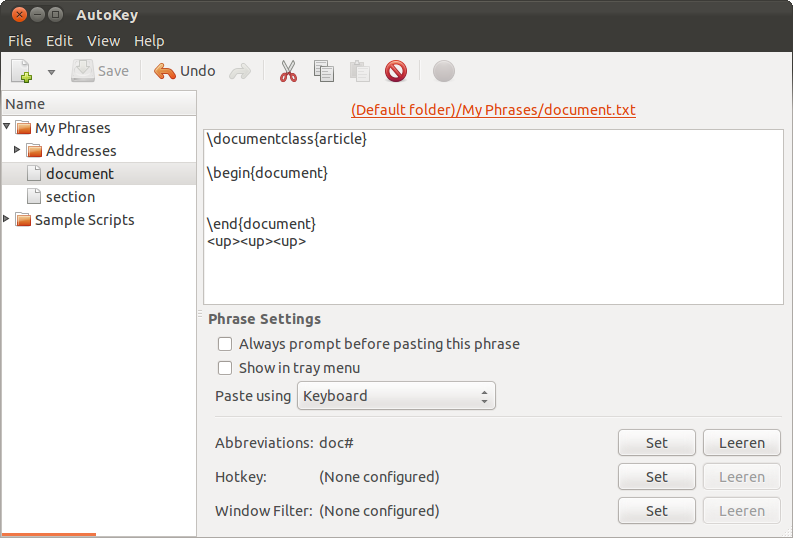
\includegraphics[width=0.85\textwidth]{autokey1}
\caption{Autokey Screenshot}
\end{center}
\end{figure}

\subsection{TextExpander (Mac OS)}

TextExpander für Mac OS X, siehe Abbildung \ref{fig:tx}, ist mit einem Preis von \$\,34,95 die einzige kommerzielle Lösung dieses Artikels. Neben der Ex\-pan\-sion von Tastenkürzeln kann TextExpander mit Datumswerten rechnen oder AppleScript/Shell-Skripte ausführen. Auf der OS~X Plattform gilt TextExpander als \emph{die} Referenz. Es gibt sogar eine Version für iOS, die aber leider auf die individuelle Unterstützung durch jede einzelne App angewiesen ist.

\begin{figure}[h]
\begin{center}
\fbox{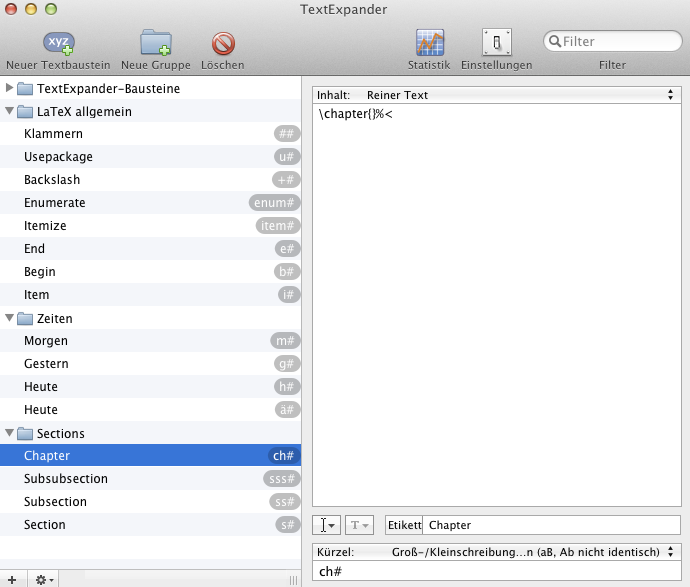
\includegraphics[width=0.8\textwidth]{textexpander1}}
\caption{Textexpander Screenshot (Mac OS~X)}\label{fig:tx}
\end{center}
\end{figure}


\subsection{Autohotkey (Windows)}

\ahk gibt es seit mittlerweile zehn Jahren, es steht unter \url{www.autohotkey.com} zum Download bereit. Wird \ahk nach der Installation gestartet, so fragt es nach, ob es eine entsprechende \texttt{.ahk} Datei im Home-Verzeichnis des Nutzers erstellen soll. Alternativ kann man eine \texttt{.ahk} Datei auch an beliebiger Stelle ablegen und eine Verknüpfung im Autostart-Ordner anlegen, sodass beim Systemstart \ahk automatisch lädt. Beim Autor liegt diese Datei in der Dropbox, damit alle vorhandenen Windows-Rechner stets die aktuelle Version der Kürzel haben.

Die grafische Oberfläche, siehe Abbildung \ref{fig:ahk}, ist recht schlicht. Über das Kontextmenü der Applikation im System-Tray lässt sich das Skript editieren, neu laden oder pausieren. Außerdem lässt sich der \enquote{Window Spy} starten, mit dessen Hilfe man ermitteln kann, an welchen Koordinaten sich die Maus befindet oder mit welchem Namen/Typ die einzelnen offenen Fenster im \ahk-Code angesprochen werden können.

\begin{figure}[h]
\begin{center}
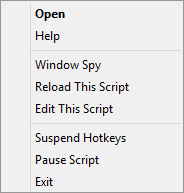
\includegraphics[width=0.35\textwidth]{AutoHotkey_soft}
\caption{Autohotkey Kontextmenü}\label{fig:ahk}
\end{center}
\end{figure}

Ruft man den edit-Befehl auf, so startet \ahk Notepad.exe. Wer mehr Editor-Funktionalität benötigt, dem sei SciTE4AutoHotkey\footnote{\url{http://fincs.ahk4.net/scite4ahk/}} empfohlen, das Funktionen wie Syntax-Highlighting und Auto-Completion bietet.

Der Funktionsumfang von \ahk ist ausgesprochen hoch, neben den in diesem Artikel besprochenen Tastenkürzeln bietet \ahk eine komplette Skriptsprache, mit der neben der Automatisierung vieler Windows-Funktionen sogar grafische Benutzeroberflächen gestaltet werden können.

\section{Kürzel-Expansion und mehr mit \ahk}

Im zweiten Teil dieses Artikels soll es um die konkrete Definition verschiedener \TeX nischer Kürzel mit \ahk unter Windows gehen, die gezeigten Funktionen sollten sich aber größtenteils auch auf den anderen Plattformen umsetzen lassen.

Listing \ref{ahk:eins} zeigt einfache Beispiele, wie die Tastenkürzel -- auch \enquote{Hotstrings} genannt -- definiert werden müssen, damit aus \texttt{s\#}, \texttt{ss\#} und \texttt{sss\#} entsprechende Gliederungsbefehle werden. Die Kürzel werden dabei so gesetzt, dass unmittelbar nach der Eingabe des Kürzels ersetzt wird. 

\begin{lstlisting}[frame=single,caption={\textbackslash section-Expansionen},label={ahk:eins}]
:*:s#::\section{{}{}}{LEFT}
:*:ss#::\subsection{{}{}}{LEFT}
:*:sss#::\subsubsection{{}{}}{LEFT}
\end{lstlisting}

Es gibt auch die Möglichkeit, erst nach einem Auslöse-Zeichen (wie Leer- oder Satzzeichen) zu expandieren, mehr dazu im Hilfesystem.\footnote{\url{www.autohotkey.com/docs/Hotstrings.htm}}

Da geschweifte Klammern für Autohotkey aktive Zeichen darstellen (die Befehle zum Bewegen des Cursors stehen beispielsweise in geschweiften Klammern) müssen geschweifte Klammern, die in unserem \LaTeX-Dokument auftauchen sollen, entsprechend ausgezeichnet werden. Das \texttt{\{LEFT\}} am Ende schließlich weist \ahk an, den Cursor um ein Zeichen nach links zu bewegen. Schon dieses einfache Beispiel zeigt, mit \ahk lässt sich jede Menge Tipp-Arbeit sparen!

Tabelle \ref{tab:ahktw} zeigt die Kürzel, die ich für mich definiert habe und als sinnvoll erachte. Das sichtbare Leerzeichen \textvisiblespace\ zeigt dabei, wo der Cursor nach der Expansion steht.

\begin{table}[h]
\begin{center}
\begin{tabular}{p{6.25cm}p{4cm}}   \\ \toprule
Modifier & Beschreibung \\ \midrule
\# & Windows \\
! & Alt \\
+ & Shift \\
\textasciicircum & Control-Taste (Strg) \\
\bottomrule \end{tabular}
\caption{Nützliche Kürzel für \LaTeX} \label{tab:mods}
\end{center}
\end{table}


\begin{longtable}{p{6.25cm}p{4cm}} \caption[Verschiedene Kürzel]{Nützliche Kürzel für \LaTeX} \label{tab:ahktw}  \\ \toprule
Kürzel & Expansion \\ \midrule
\verb|:*:c#::\chapter{{}{}}{LEFT}| & \textbackslash chapter\{\textvisiblespace \}\\
\verb|:*:s#::\section{{}{}}{LEFT}| & \textbackslash section\{\textvisiblespace \}\\
\verb|:*:ss#::\subsection{{}{}}{LEFT}| & \textbackslash subsection\{\textvisiblespace \}\\
\verb|:*:sss#::\subsubsection{{}{}}{LEFT}| & \textbackslash subsubsection\{\textvisiblespace \}\\
\verb|:*:b#::\begin{{}{}}{LEFT}| & \textbackslash begin\{\textvisiblespace \} \\
\verb|:*:e#::\begin{{}{}}{LEFT}| & \textbackslash end\{\textvisiblespace \} \\
\verb|:*:i#::\item{Space}| & \textbackslash item \textvisiblespace \\
\verb|:*:l#::\label{{}{}}{LEFT}| & \textbackslash label\{\textvisiblespace\} \\
\verb|:*:r#::\label{{}{}}{LEFT}| & \textbackslash ref\{\textvisiblespace\} \\
\verb|:*:(::(){LEFT}| & (\textvisiblespace) \\
\verb|:*:{::{{}{}}{LEFT}| & \{\textvisiblespace\} \\ 
\verb|:*:[::[]{LEFT}| & [\textvisiblespace] \\
\bottomrule \end{longtable}

Nicht nur \enquote{normale} Tasten lassen sich über \ahk ansteuern. Tabelle~\ref{tab:mods} zeigt einige wichtige \enquote{Keyboard-Modifier}, die vollständige Liste ist unter \url{www.autohotkey.com/docs/Hotkeys.htm#Symbols} verfügbar:

Listing \ref{ahk:fkeying} zeigt die praktische Anwendung. Für die F3- bzw. F4-Taste werden kurze Programme definiert, die aktuell markierten Text in die Zwischenablage kopieren, den \verb|\emph{}| bzw. \verb|\enquote{}| ins Dokument setzen und den Text aus der Zwischenablage an der richtigen Stelle wieder einfügen. Somit lassen sich Funktionen definieren, die in der eigentlichen Software nicht vorhanden oder nur umständlich verfügbar sind.

\begin{lstlisting}[frame=single,caption={Programmierung der F-Tasten mit \ahk},label={ahk:fkeying}]
F3::
Send ^c
Send \emph{{}{}}{LEFT}
Send ^v
Return

F4::
Send ^c
Send \enquote{{}{}}{LEFT}
Send ^v
Return
\end{lstlisting}

Listing \ref{ahk:dupe} zeigt zwei Befehle, die von mir in \TeX works schmerzlich vermisste Funktionen nachrüsten: das Löschen einer Zeile über \verb|Strg-k| und die Duplikation einer Zeile über \verb|Strg-d|.

\begin{lstlisting}[frame=single,caption={Zeilen duplizieren und löschen},label={ahk:dupe}]
#IfWinActive ahk_class QWidget
{
^k:: 
Send {HOME}
Send {SHIFT}+{END}
Send {DEL 2}
return

^d::
Send {HOME}
Send {SHIFT}+{END}
Send ^c
ClipWait, 2
Send {END}
Send {ENTER}
Send ^v
return
}
#IfWinActive 
\end{lstlisting}

\section{Oberflächen mit \ahk}

Zum Abschluss des Artikels zeigt Listing \ref{ahk:gui} noch ein relativ einfaches Script für die Programmierung einer grafischen Oberfläche. Es erzeugt über die Tastenkombination \verb|Alt+e| ein grafisches Menü, in dem der Nutzer eine Zeichenkette der Form \verb|UmgebungZahl| eingeben kann. Diese Zeichenkette wird dann intern über einen regulären Ausdruck in \enquote{Umgebung} und \enquote{Zahl} geteilt. \enquote{Umgebung} wird dann mittels \verb|\begin/\end| als \LaTeX-Umgebung ins Dokument geschrieben; es werden  \enquote{Zahl} verschiedene \verb|\item| Befehle ausgegeben und der Cursor hinter dem ersten \verb|\item| positioniert.

\begin{figure}[h]
\begin{center}
\fbox{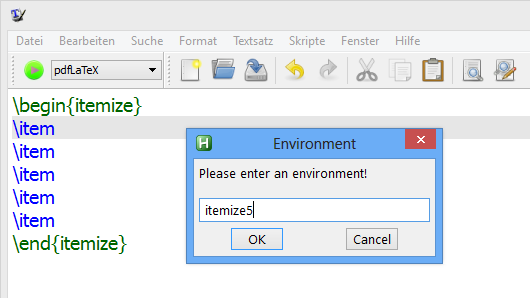
\includegraphics[width=0.8\textwidth]{gui}}
\caption{Grafische Oberfläche aus Listing \ref{ahk:gui}}\label{fig:gui}
\end{center}
\end{figure}

\section{Fazit}

Wer einmal mit einem Text Expander gearbeitet hat, lernt sehr schnell die Annehmlichkeiten dieser Werkzeuge schätzen. Mit wenigen Schritten lassen sich Kürzel definieren, die schon nach kurzer Eingewähnung erheblich Zeit sparen können und dem Nutzer mehr Zeit geben, sich auf das Wesentliche -- den Text -- zu konzentrieren.

Die genutzte Autohotkey-Datei steht unter \url{www.uweziegenhagen.de} zur Verfügung, für Kommentare und Anregungen bin ich stets dankbar.

\begin{lstlisting}[frame=single,caption={Oberfläche mit \ahk},basicstyle={\ttfamily\footnotesize},label={ahk:gui}]
!e::
InputBox, UserEnv, Environment, Please specify an environment!, , 240, 120
If ErrorLevel return
Else 
if( RegExMatch(UserEnv, "(.*?)(\d+)$", splitted) ) {
	Send \begin{{}%splitted1%{}}{Enter}
		Loop %splitted2% {
			Send \item {Enter}}
	Send \end{{}%splitted1%{}}{Up}
	count2 := splitted2 - 1 
	Loop %count2% {
		Send {Up}
	}} 
Else 
	Send \begin{{}%UserEnv%{}}{Enter 2}\end{{}%UserEnv%{}}{Up}
return
\end{lstlisting}



\end{document}